\documentclass[11pt]{article}

% ---- packages (all standard; compiles on Overleaf or any TeX Live) ----
\usepackage[utf8]{inputenc}
\usepackage[T1]{fontenc}
\usepackage[margin=1in]{geometry}
\usepackage{amsmath,amssymb}
\usepackage{booktabs}
\usepackage{graphicx}
\usepackage{xcolor}
\usepackage{listings}
\usepackage{caption}
\usepackage{enumitem}
\usepackage[colorlinks=true,linkcolor=blue,citecolor=blue,urlcolor=blue]{hyperref}

\definecolor{codebg}{rgb}{0.96,0.96,0.96}
\lstset{
  basicstyle=\ttfamily\small,
  backgroundcolor=\color{codebg},
  breaklines=true,
  frame=single,
  columns=fullflexible,
  showstringspaces=false
}

\title{\textbf{LABAD: Behavioral Bifurcation Detection for Insider Threats}\\
\large An LSTM-Autoencoder UEBA Pipeline with Online Changepoint Onset Localization}
\author{Yash Yadav}
\date{\today}

\begin{document}
\maketitle

\begin{abstract}
\noindent
Most user-and-entity behavior analytics (UEBA) systems answer a single
question --- \emph{is this user anomalous?} --- and report an AUC. The
question a security analyst actually asks is \emph{when did the compromise
begin?}, because that scopes the investigation. LABAD is an insider-threat
detection pipeline on the CERT r4.2 dataset that answers both. An LSTM
autoencoder trained only on benign behavior produces per-user anomaly
scores; a Neyman--Pearson rule calibrates the operating point to a fixed
false-positive budget; and---the central contribution---\emph{Bayesian
Online Changepoint Detection (BOCPD)} localizes the onset of malicious
activity by treating each user's behavior as a dynamical system and
detecting the moment its statistical regime changes: a behavioral
\emph{bifurcation}. The system reaches AUC $0.87$ and $100\%$
precision@10 for detection, and localizes the onset of abrupt insiders
(CERT scenario~1) to within $\pm 7$ days in $\approx 80\%$ of cases, a
median of $3$ days, typically $1$--$2$ days \emph{before} the labeled
onset. We additionally report negative results---CUSUM and critical-slowing-down
detectors fail here, and we root-cause the failure to the
\emph{signal} rather than the algorithm: the scalar reconstruction error
dilutes a $151\times$ single-feature spike into a $1.03\times$ non-event.
The pipeline is containerized (Docker, CPU-only $2.93$\,GB image) and
experiment-tracked (MLflow).
\end{abstract}

\section{Introduction}

Insider threats are among the costliest and hardest-to-detect security
risks: the actor already has legitimate access, so signature- and
rule-based controls do not fire. UEBA reframes the problem as anomaly
detection over behavior. The dominant academic approach---an LSTM or
autoencoder over the CERT insider-threat dataset---is by now well-trodden,
and typically stops at a discrimination metric.

LABAD's thesis is that the operationally valuable output is not just a
risk score but an \emph{onset timestamp}. We formalize ``when did the
compromise begin'' as changepoint detection on each user's anomaly-score
time series, grounded in a dynamical-systems view: a benign user occupies
a stable behavioral regime, and going rogue is a \emph{bifurcation}---a
sharp qualitative transition to a new regime. BOCPD detects exactly this,
online.

\paragraph{Contributions.}
\begin{enumerate}[itemsep=2pt,topsep=2pt]
  \item An end-to-end UEBA pipeline: feature engineering $\rightarrow$
        LSTM-autoencoder anomaly scoring $\rightarrow$ Neyman--Pearson
        calibration $\rightarrow$ BOCPD onset detection $\rightarrow$
        RAG-grounded LLM threat reports, containerized and tracked.
  \item A from-scratch BOCPD implementation with a corrected changepoint
        readout, and an evaluation showing onset localization to a median
        of $3$ days on abrupt insiders.
  \item Rigorous \emph{negative} results: CUSUM and critical slowing down
        do not improve on BOCPD, root-caused to signal autocorrelation and
        scalar-score dilution rather than detector choice.
  \item A per-feature ablation that recovers the diluted signal and adds
        feature-level explainability.
\end{enumerate}

\section{Data and Feature Engineering}

We use \textbf{CERT r4.2}, a synthetic but richly simulated insider-threat
corpus ($\approx 16$\,GB of raw logs across logon, device/USB, file,
email, and HTTP activity), with ground-truth incidents in
\texttt{insiders.csv}. After filtering to release~4.2 there are $70$
labeled malicious users across three attack scenarios.

Raw events are aggregated into \textbf{per-user, per-day} feature vectors
of $18$ behavioral dimensions: logon counts and after-hours/weekend
logons, first/last activity hour, USB connect counts (and after-hours
USB), file access and after-hours file access, executable access, unique
files, email counts (external, with-attachment, average size), HTTP
counts, job-site visits, and cloud-storage visits. A day is the smallest
unit at which behavior is stable enough to compare.

\paragraph{Evaluation discipline.} We split \emph{at the user level}
(80\% of benign users for training; the remaining benign users plus all
malicious users for test) and fit the feature scaler on training users
only. A row-level split would let the model memorize a user's baseline
from training rows and trivially flag the test rows of the same user---an
unrealistic UEBA evaluation.

\section{Anomaly Detection Model}

\subsection{Architecture and training}
The detector is an \textbf{LSTM autoencoder} (encoder hidden dimension
$128$, latent $64$, $2$ layers, dropout $0.2$; $838{,}098$ parameters). It
consumes $30$-day sliding windows of the $18$-dimensional features
($351{,}168$ training sequences) and is trained \emph{only on benign
users} to reconstruct normal behavior. Anomalous sequences lie off the
learned manifold and reconstruct poorly.

We minimize mean-squared reconstruction error with Adam ($\text{lr}=10^{-3}$),
gradient clipping at $1.0$, and a \texttt{CosineAnnealingWarmRestarts}
schedule ($T_0=30,\,T_{\text{mult}}=2,\,\eta_{\min}=10^{-5}$) stepped
per-batch, for $50$ epochs (best validation MSE $0.394$). Training is
tracked in MLflow (Section~\ref{sec:mlops}).

\begin{figure}[t]
  \centering
  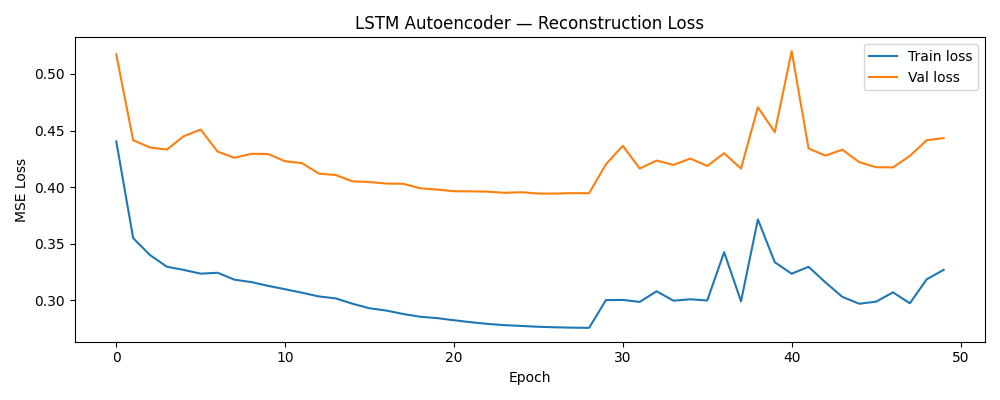
\includegraphics[width=0.8\linewidth]{data/processed/training_curve.png}
  \caption{Training and validation reconstruction loss. The periodic
  bumps are the cosine warm restarts; the best checkpoint is retained.}
  \label{fig:train}
\end{figure}

\subsection{Anomaly score}
For a window $x$, the scalar anomaly score is the reconstruction error
averaged over both time and features,
\begin{equation}
  s(x) \;=\; \frac{1}{T F}\sum_{t=1}^{T}\sum_{f=1}^{F}\bigl(x_{tf}-\hat{x}_{tf}\bigr)^2 ,
  \label{eq:scalar}
\end{equation}
with $T=30$ and $F=18$. Per-user scores aggregate window scores by
maximum, mean, top-$3$ mean, and $95$th percentile.

\section{Neyman--Pearson Calibration}

A SOC has fixed analyst capacity, so the relevant constraint is a fixed
false-positive rate $\alpha$, not an arbitrary threshold. We calibrate the
decision threshold $\tau$ on \emph{held-out benign} scores by the
empirical $(1-\alpha)$ quantile,
\begin{equation}
  \tau \;=\; Q_{1-\alpha}\bigl(\{s : \text{benign}\}\bigr),
  \qquad \widehat{\Pr}(s>\tau \mid \text{benign}) \approx \alpha .
\end{equation}
This is the Neyman--Pearson criterion: maximize detection (true-positive
rate) subject to $\text{FPR}\le\alpha$. At $\alpha=1\%$ we obtain
$\tau=2.19$.

\section{Behavioral Bifurcation Detection (BOCPD)}
\label{sec:bocpd}

\subsection{The model}
We run BOCPD \cite{adams2007} on each user's daily anomaly-score series.
The core latent variable is the \emph{run length} $r_t$---days since the
last changepoint. BOCPD maintains the full posterior $P(r_t \mid x_{1:t})$
online. At each day the run either grows ($r_t=r_{t-1}+1$) or resets
($r_t=0$). With hazard $H=1/\lambda$ (we use $\lambda=50$) and a predictive
$\pi_r=P(x_t\mid r_{t-1}=r)$, the recursion is
\begin{align}
  P(r_t = r{+}1, x_{1:t}) &= P(r_{t-1}=r, x_{1:t-1})\,\pi_r\,(1-H), \\
  P(r_t = 0,\; x_{1:t})   &= \textstyle\sum_r P(r_{t-1}=r, x_{1:t-1})\,\pi_r\,H .
\end{align}
The predictive is Student-$t$ via a Normal--Inverse--Gamma conjugate prior
with unknown mean \emph{and} variance, so the detector adapts to each
user's baseline volatility:
$\pi_r = \mathrm{St}\!\left(x_t;\,2\alpha_r,\,\mu_r,\,
\sqrt{\beta_r(\kappa_r{+}1)/(\alpha_r\kappa_r)}\right)$.

\subsection{A corrected changepoint readout}
A common but incorrect way to declare changepoints is to threshold
$R[0,t]\equiv P(r_t=0)$. This carries \emph{no information}: with
$S=\sum_r P(r_{t-1}{=}r,x_{1:t-1})\pi_r$, normalization gives
\begin{equation}
  R[0,t] \;=\; \frac{H\,S}{(1-H)S + H\,S} \;=\; H ,
\end{equation}
i.e. $R[0,t]$ equals the hazard at \emph{every} step regardless of the
data. The regime change instead manifests as the run-length posterior
\emph{collapsing onto short run lengths}. We therefore read off
\begin{equation}
  c_t \;=\; \Pr(r_t \le w) \;=\; \sum_{r=0}^{w} R[r,t],
  \qquad w=5,
\end{equation}
and flag an onset at the first upward crossing of $c_t$ through $0.5$ after
a burn-in. On a synthetic mean-shift this collapses the MAP run length from
$50$ to $1$ at the true changepoint and fires $c_t:0.08\!\to\!0.96$ with a
one-day online lag.

\subsection{Results}
Onset-detection accuracy is strongly \emph{scenario-dependent}, exactly as
the bifurcation framing predicts (Table~\ref{tab:bocpd}). On scenario~1
(abrupt: after-hours access $+$ removable media $+$ exfiltration) BOCPD
localizes the onset to within $\pm 7$ days in $\approx 80\%$ of cases, a
median of $3$ days, with a mean signed latency of $-2$ days (i.e.\ it
tends to fire just \emph{before} the labeled onset as behavior ramps up).
On scenario~2 (gradual job-site browsing then exfiltration) it is weak: a
slow drift produces no sharp run-length collapse. This is correct
behavior, not a defect---a bifurcation is by definition a sharp
transition.

\begin{table}[t]
  \centering
  \caption{Onset localization within $\pm 7$ days by CERT scenario (BOCPD).}
  \label{tab:bocpd}
  \begin{tabular}{lcc}
    \toprule
    CERT scenario & Within $\pm 7$ days & Character \\
    \midrule
    1 (after-hours $+$ USB $+$ exfil) & $\approx 24$--$25/30$ ($80\%$) & sharp shift \\
    2 (job-site surfing $\rightarrow$ exfil) & $1/30$ & gradual drift \\
    3 (disgruntled sysadmin) & $4/10$ & mixed \\
    \bottomrule
  \end{tabular}
\end{table}

\begin{figure}[t]
  \centering
  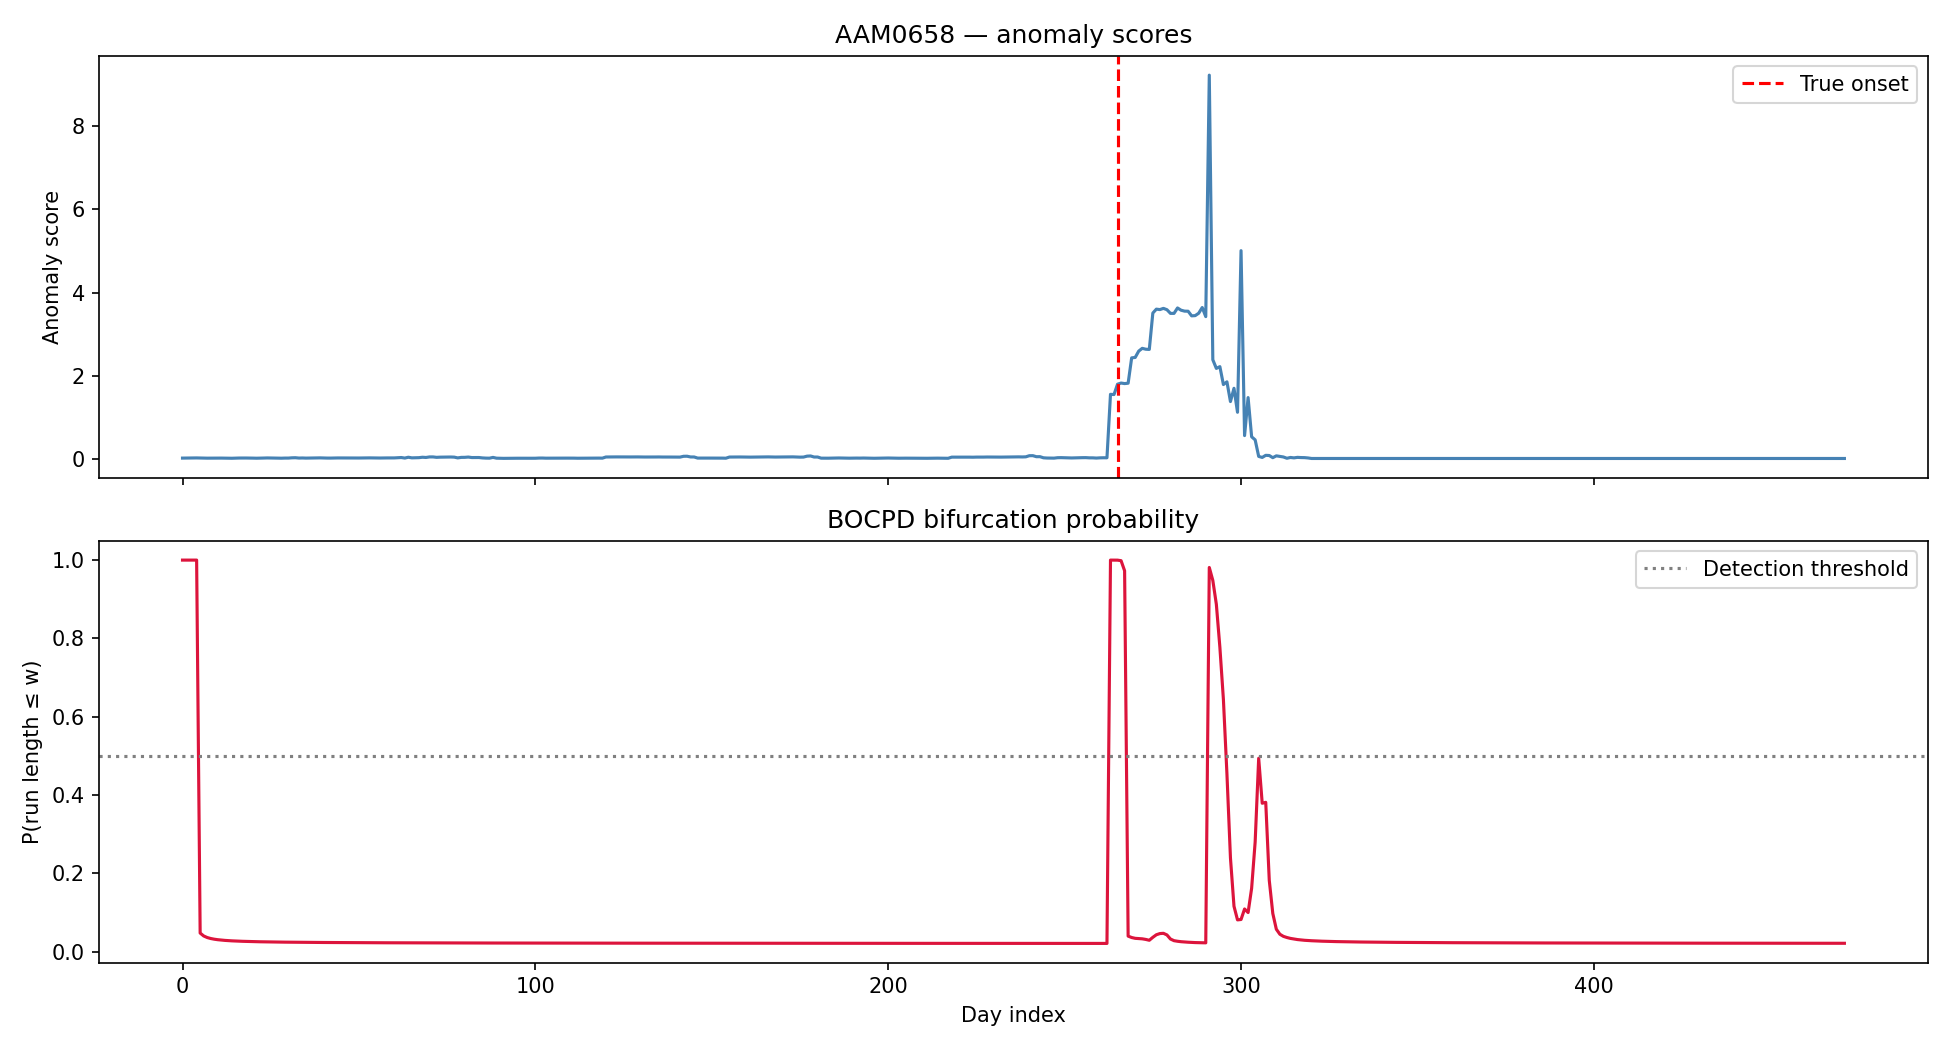
\includegraphics[width=0.9\linewidth]{data/processed/bocpd_example.png}
  \caption{A scenario-1 user. Top: daily anomaly score with the labeled
  onset (dashed). Bottom: the run-length collapse signal $c_t$ spiking at
  the regime change.}
  \label{fig:bocpd}
\end{figure}

\section{Negative Results and Root-Cause Analysis}

To target the gradual-drift failure we added two principled complements
and evaluated them honestly (first causal alarm; $|\text{latency}|>14$
days counts as a miss).

\paragraph{CUSUM and critical slowing down both fail.} Under causal
evaluation both detectors false-alarm almost immediately for every user
(median latency $-84$ to $-182$ days), and scenario~2 detection is
$0/30$ across all transforms (raw, log, differenced). The cause is the
\emph{signal}: overlapping $30$-day windows make the score series heavily
autocorrelated (lag-$1$ autocorrelation $0.83$--$0.99$), violating the
near-independence both methods assume, and the near-constant early window
yields a degenerate baseline standard deviation ($\sim 10^{-3}$) that any
threshold trips. BOCPD's sequential Bayesian model is comparatively robust
to this structure.

\paragraph{The bottleneck is the scalar score, not the detector.} The
scalar in Eq.~\eqref{eq:scalar} averages over all $18$ features. At onset,
the mean score rises $8.81\times$ for scenario~1 but only $1.03\times$ for
scenario~2---effectively no event. Yet the underlying behavior \emph{does}
change: a single feature's reconstruction error spikes $\sim 151\times$
(\texttt{exe\_access\_count}), and raw \texttt{job\_site\_visits} goes from
near-zero to active. The averaging in Eq.~\eqref{eq:scalar} destroys a
strong single-dimension signal. \emph{One cannot detect what the score does
not encode.}

\section{Per-Feature Ablation}

We therefore score per feature, averaging over time only,
\begin{equation}
  s_f(x) \;=\; \frac{1}{T}\sum_{t=1}^{T}\bigl(x_{tf}-\hat{x}_{tf}\bigr)^2 ,
  \qquad f=1,\dots,F,
\end{equation}
yielding $18$ error series per user, and run BOCPD per feature with a
coordinated-collapse fusion (flag when $\ge 2$ features collapse together,
which suppresses single-feature noise). This \emph{matches} the scalar on
scenario~1 ($25/30$ within $\pm 7$ days, median $-3$ days) and---crucially---
identifies \emph{which} behaviors drove the alert, adding explainability the
scalar cannot. It confirms the dilution diagnosis quantitatively
(Table~\ref{tab:dilution}). Recovering gradual (scenario~2) onsets remains
open: their signal lives in $1$--$2$ \emph{sparse} features, so any
single-feature trigger false-alarms across $18$ noisy dimensions---a sparse
multivariate online-changepoint problem we leave to future work.

\begin{table}[t]
  \centering
  \caption{Score change at onset (30 days before vs.\ after).}
  \label{tab:dilution}
  \begin{tabular}{lcc}
    \toprule
    Scenario & Scalar score ratio & Max single-feature ratio \\
    \midrule
    1 (abrupt) & $8.81\times$ & $183\times$ \\
    2 (gradual) & $1.03\times$ (non-event) & $151\times$ (\texttt{exe\_access\_count}) \\
    \bottomrule
  \end{tabular}
\end{table}

\section{LLM Threat Reports}

For the highest-risk users, LABAD generates analyst-ready reports. A FAISS
index over the MITRE ATT\&CK knowledge base retrieves techniques relevant
to each user's behavioral evidence (RAG), and a \emph{local} LLM
(Ollama, \texttt{llama3.1:8b}) writes a structured report---threat summary,
severity, ATT\&CK mapping, recommended actions, confidence---under an
anti-hallucination instruction to use only retrieved context. Running the
model locally is a deliberate design choice: behavioral logs are sensitive,
and an air-gapped, zero-external-API pipeline is a requirement for
real deployments.

\section{Detection Results}

\begin{table}[t]
  \centering
  \caption{Detection performance (user-level, max aggregation; $70$
  malicious / $256$ test users).}
  \label{tab:detection}
  \begin{tabular}{lc}
    \toprule
    Metric & Value \\
    \midrule
    AUC-ROC & $0.87$ \\
    Average Precision & $0.72$ \\
    Malicious/benign score separation & $7.36\times$ \\
    TPR @ $10\%$ FPR & $55.7\%$ \\
    Neyman--Pearson @ $1\%$ FPR (precision / recall) & $70\%$ / $43\%$ \\
    Precision@10 (top-$3$ aggregation) & $100\%$ \\
    \bottomrule
  \end{tabular}
\end{table}

Table~\ref{tab:detection} summarizes detection. The strong
precision@10 means the top of the alert queue is almost entirely true
insiders---the property that matters for analyst triage---while the
moderate recall at $1\%$ FPR reflects the genuine difficulty of the
gradual scenarios.

\begin{figure}[t]
  \centering
  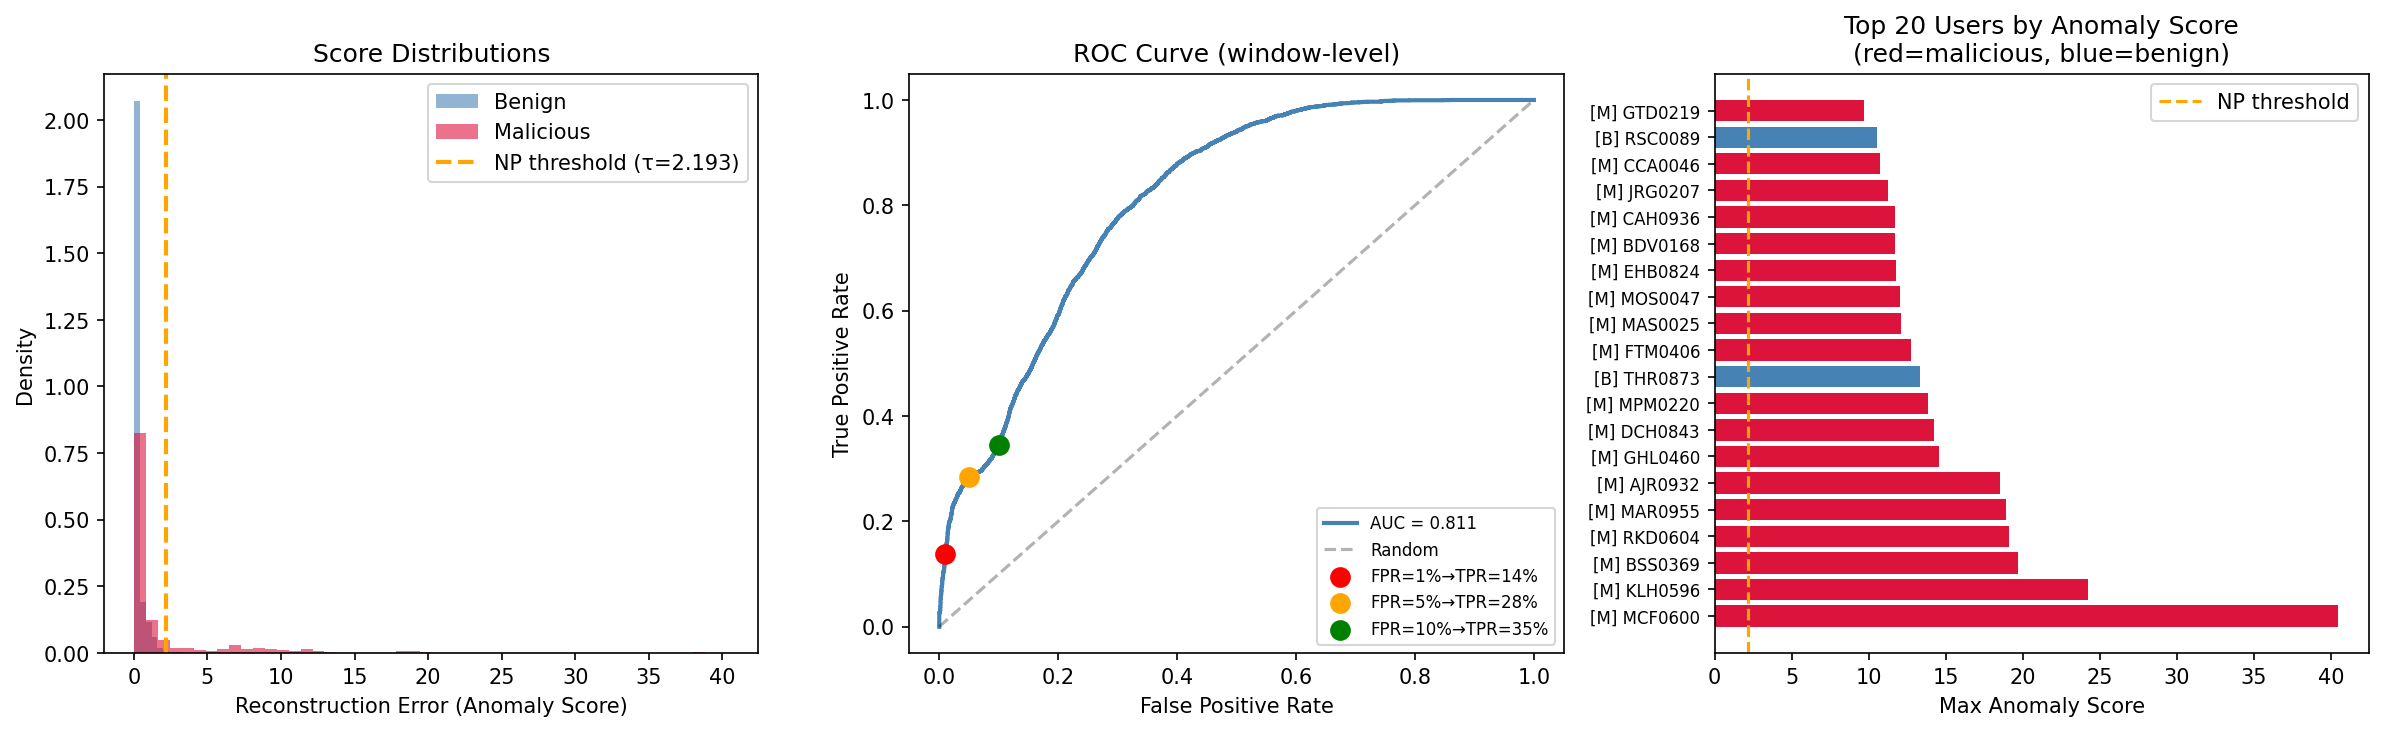
\includegraphics[width=\linewidth]{data/processed/anomaly_distributions.png}
  \caption{Score distributions (benign vs.\ malicious), ROC with
  Neyman--Pearson operating points, and the top-scored users.}
  \label{fig:dist}
\end{figure}

\section{System and Reproducibility}
\label{sec:mlops}

The pipeline is containerized with Docker and \texttt{docker-compose} (an
\texttt{ollama} service plus the application). The image is CPU-only and
$2.93$\,GB: the default PyTorch wheel bundles a multi-gigabyte CUDA stack
that is dead weight in a CPU container, so we install from the PyTorch CPU
index. Training runs are tracked in MLflow (parameters, per-epoch metrics,
model and curve artifacts) against a SQLite backend, viewable with
\texttt{mlflow ui}.

\section{Limitations and Future Work}
\begin{itemize}[itemsep=2pt,topsep=2pt]
  \item \textbf{Gradual insiders.} Scenario~2 onset detection is unsolved;
        the signal is recoverable per-feature but requires sparse
        multivariate online changepoint methods.
  \item \textbf{Early warning.} Critical slowing down (rising variance and
        autocorrelation before a tipping point) could \emph{predict} onset
        rather than detect it, on a decorrelated signal.
  \item \textbf{Dataset.} CERT is synthetic; transfer to real telemetry is
        the key external-validity question.
  \item \textbf{Beyond human insiders.} The core capability---detect when
        an entity's behavior changes regime on a stream of its actions---
        applies directly to monitoring autonomous AI agents for
        compromise, prompt-injection, or goal-drift.
\end{itemize}

\section{Conclusion}

LABAD shows that an insider-threat pipeline can answer \emph{when}, not
just \emph{whether}, by detecting behavioral bifurcations with online
changepoint detection. It localizes abrupt-insider onsets to a median of
three days, reaches AUC $0.87$ and $100\%$ precision@10, and---through
honest negative results---identifies the true bottleneck as signal
representation rather than detector choice. The dynamical-systems framing
is not decoration: the quantity whose collapse signals the bifurcation is
literally the run-length posterior the algorithm computes.

\begin{thebibliography}{9}
\bibitem{adams2007} R.~P.~Adams and D.~J.~C.~MacKay.
  \emph{Bayesian Online Changepoint Detection}. arXiv:0710.3742, 2007.
\bibitem{cert} J.~Glasser and B.~Lindauer.
  \emph{Bridging the Gap: A Pragmatic Approach to Generating Insider Threat Data}.
  IEEE Security and Privacy Workshops, 2013.
\bibitem{scheffer2009} M.~Scheffer et al.
  \emph{Early-warning signals for critical transitions}. Nature 461, 2009.
\bibitem{mitre} MITRE ATT\&CK\textsuperscript{\textregistered} Framework.
  \url{https://attack.mitre.org}.
\end{thebibliography}

\end{document}
